\newcommand{\figuraAtmosferaIsotermica}{%
\begin{figure}[htbp]
    \centering
    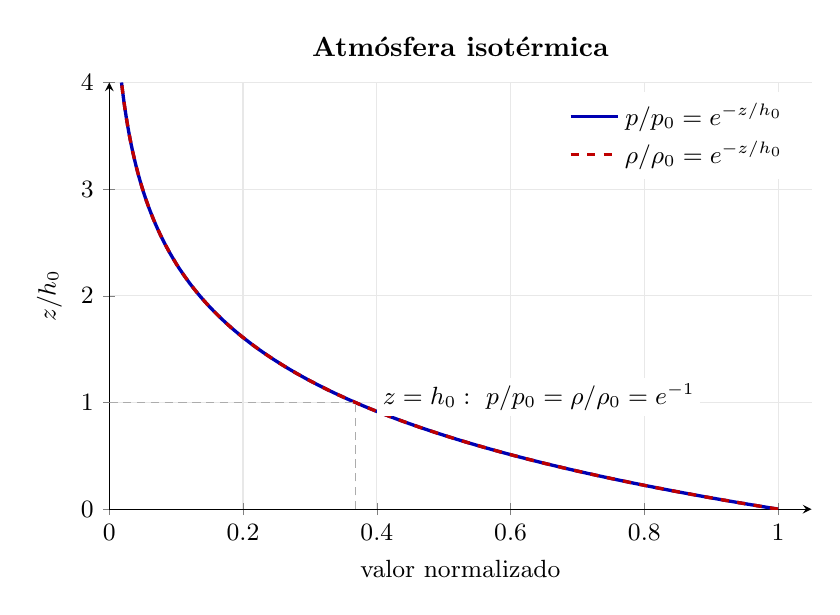
\begin{tikzpicture}[font=\small]
        \begin{axis}[
            width=10.5cm,
            height=7.0cm,
            xmin=0,
            xmax=1.05,
            ymin=0,
            ymax=4.0,
            xlabel={valor normalizado},
            ylabel={$z/h_0$},
            axis lines=left,
            grid=major,
            major grid style={gray!18},
            legend style={
                at={(0.98,0.98)},
                anchor=north east,
                draw=none,
                fill=white
            },
            title={Atmósfera isotérmica},
            title style={font=\bfseries}
        ]
            \addplot[very thick,blue!70!black,samples=180,domain=0:4]
                ({exp(-x)},x);
            \addlegendentry{$p/p_0=e^{-z/h_0}$}

            \addplot[very thick,red!75!black,dashed,samples=180,domain=0:4]
                ({exp(-x)},x);
            \addlegendentry{$\rho/\rho_0=e^{-z/h_0}$}

            \draw[densely dashed,gray!65]
                (axis cs:0,1)--(axis cs:0.368,1);
            \draw[densely dashed,gray!65]
                (axis cs:0.368,0)--(axis cs:0.368,1);
            \node[anchor=west,fill=white,inner sep=2pt]
                at (axis cs:0.40,1.05)
                {$z=h_0:\ p/p_0=\rho/\rho_0=e^{-1}$};
        \end{axis}
    \end{tikzpicture}
    \caption{En una atmósfera isotérmica, la presión y la densidad decrecen
    exponencialmente con la misma altura de escala $h_0=RT_0/g_0$.}
    \label{fig:atmosfera-isotermica}
\end{figure}%
}